\documentclass[12pt,a4paper]{article}
\usepackage{amsmath}
\usepackage{amsfonts}
\usepackage{amssymb}
\usepackage{graphicx}
\usepackage{url}
\usepackage[left=2cm,right=2cm,top=2cm,bottom=2cm]{geometry}

\author{Taher S A}
\title{Mass-energy equivalence relationship}

\date{February 5, 2023}

\begin{document}

\maketitle

\section{me22b002}

Albert Einstein’s (Figure~\ref{pic}) paper “Does the Inertia of a Body Depend Upon Its Energy Content?” was published in the journal “Annalen der Physik” on November 21, 1905.

\begin{figure}[h]
	\begin{center}
		\framebox{
			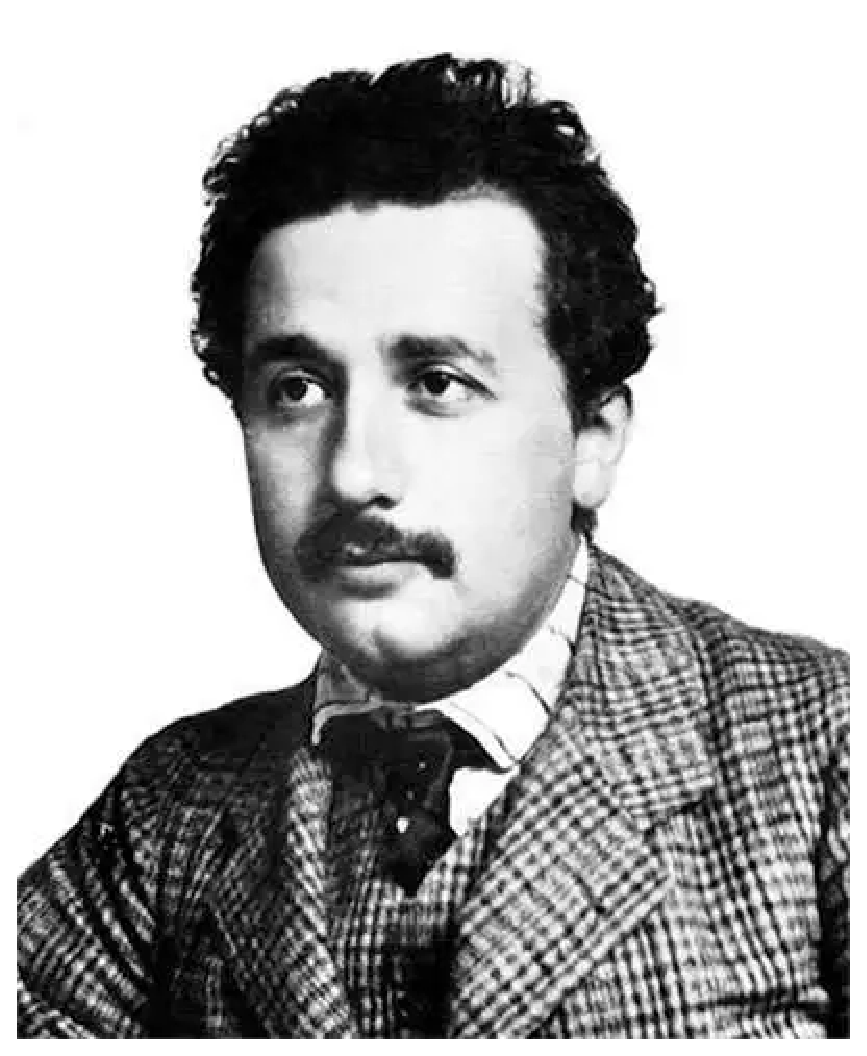
\includegraphics[scale=0.3]{img.eps}
		}
	\end{center}
	\caption{What you can't imagine, you can't discover. -Albert Einstein}
	\label{pic}
\end{figure}

The paper revealed the relationship between energy and mass that would eventually lead to the famous mass-energy equivalence formula 

\begin{equation}
    E = mc^2
    \label{main_eqn}
\end{equation}

where E is the body's kinetic energy, m is the increased relativistic mass of the body and c is the speed of light.

\begin{itemize}
    \item Name: Taher S A
    \item Github User ID: Taher-SA
\end{itemize}

This article is referred from EDN~\cite{edn}.  

\bibliography{refs}
\bibliographystyle{alpha}

\end{document}